% Seccion_Dinamica.tex


\section{Dinámica}
\label{sec:dinamica}


\subsection{Conceptos básicos}
La \emph{dinámica} estudia las causas del movimiento. Las cantidades más importantes son la masa $m$ (medida de inercia) y la fuerza $\vec{F}$ (vector que causa aceleración). La relación fundamental entre fuerza y movimiento se expresa mediante la segunda ley de Newton:


\begin{equation}\label{eq:segunda_newton}
\vec{F}_{\text{net}} = m\,\vec{a},
\end{equation}


donde $\vec{F}_{\text{net}}$ es la suma vectorial de todas las fuerzas actuantes y $\vec{a}$ es la aceleración resultante.


\subsection{Las leyes de Newton}
\begin{itemize}
\item \textbf{Primera ley (inercia):} Si la fuerza neta sobre un cuerpo es cero, su velocidad es constante (reposo o movimiento rectilíneo uniforme).
\item \textbf{Segunda ley:} Expresada en \eqref{eq:segunda_newton}. En componentes cartesianas: $\sum F_x = m a_x$, $\sum F_y = m a_y$.
\item \textbf{Tercera ley:} A toda acción corresponde una reacción igual y opuesta: si el cuerpo A ejerce $\vec{F}_{A\to B}$ sobre B, entonces B ejerce $\vec{F}_{B\to A} = -\vec{F}_{A\to B}$ sobre A.
\end{itemize}


\subsection{Diagramas de cuerpo libre (DCL)}
Para resolver problemas de dinámica, dibuja siempre el diagrama de cuerpo libre: representa el cuerpo aislado y todas las fuerzas que actúan sobre él (peso, normal, fricción, tensión, fuerza aplicada, etc.).


% Diagrama sencillo con tikz
\begin{center}
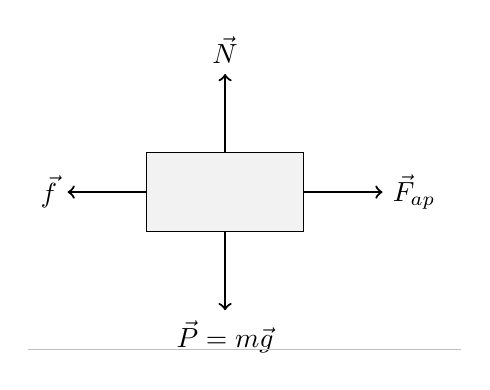
\begin{tikzpicture}[scale=1]
% bloque
\filldraw[fill=gray!10,draw=black] (0,0) rectangle (2,1);
% fuerzas
\draw[->,thick] (1,1) -- (1,2) node[above] {$\vec{N}$};
\draw[->,thick] (1,0) -- (1,-1) node[below] {$\vec{P}=m\vec{g}$};
\draw[->,thick] (2,0.5) -- (3,0.5) node[right] {$\vec{F}_{\text{ap}}$};
\draw[->,thick] (0,0.5) -- (-1,0.5) node[left] {$\vec{f}$};
% eje
\draw[gray!50] (-1.5,-1.5) -- (4,-1.5);
\end{tikzpicture}
\end{center}


\subsection{Ejemplo resuelto}
\textbf{Problema:} Un bloque de masa $m=2\,\mathrm{kg}$ está sobre una superficie horizontal con coeficiente de fricción cinética $\mu_k=0.2$. Se aplica una fuerza horizontal constante $F_{\text{ap}}=10\,\mathrm{N}$. Determina la aceleración del bloque.


\textbf{Solución:}
\begin{enumerate}
\item Fuerzas en eje $y$: $N - mg = 0 \Rightarrow N = mg$.
\item Fuerza de fricción cinética: $f_k = \mu_k N = \mu_k mg$.
\item Fuerza neta en $x$: $F_{\text{net},x} = F_{\text{ap}} - f_k = F_{\text{ap}} - \mu_k mg$.
\item Aceleración: \( a = \dfrac{F_{\text{net},x}}{m} = \dfrac{F_{\text{ap}}}{m} - \mu_k g. \)
\end{enumerate}


Sustituyendo: \( a = \dfrac{10}{2} - 0.2\cdot 9.81 \approx 5 - 1.962 = 3.038\,\mathrm{m/s^2}. \)


\subsection{Problemas propuestos}
\begin{enumerate}
\item (Fácil) Un bloque de $5\,\mathrm{kg}$ está sobre una superficie horizontal sin fricción. Se aplica una fuerza horizontal de $15\,\mathrm{N}$. Calcula la aceleración.
\item (Intermedio) Un cuerpo de $m=4\,\mathrm{kg}$ es halado por una cuerda que forma un ángulo de $30^\circ$ respecto a la horizontal con una fuerza de $20\,\mathrm{N}$ sobre una superficie con $\mu_s=0.4$ y $\mu_k=0.35$. Determina si el cuerpo se mueve y, en caso afirmativo, su aceleración.
\item (Avanzado) Plano inclinado: Un bloque de masa $m$ descansa sobre un plano inclinado de ángulo $\theta$. Considera fricción con coeficiente $\mu$. Determina la condición para que el bloque comience a deslizar y calcula la aceleración descendente si desliza.
\end{enumerate}


% Soluciones (breves)
\subsection*{Soluciones (esquema)}
\begin{itemize}
\item \textbf{1.} $a = F/m = 15/5 = 3\,\mathrm{m/s^2}$.
\item \textbf{2.} Descomponer fuerzas: componente horizontal de la tensión $T_x = 20\cos30^\circ$. Comparar con $F_{\text{fr,max}} = \mu_s N = \mu_s(mg - T_y)$; si $T_x > F_{\text{fr,max}}$ hay movimiento. Luego usar segunda ley para $a$. (Deja que el alumno haga los cálculos.)
\item \textbf{3.} Componente del peso paralelo: $mg\sin\theta$. Fuerza de fricción máxima: $\mu mg\cos\theta$. Deslizamiento si $mg\sin\theta > \mu mg\cos\theta$ (es decir, $\tan\theta > \mu$). Si desliza, $a = g(\sin\theta - \mu\cos\theta)$.
\end{itemize}


% Fin del fragmento